% !TeX root = ../main.tex
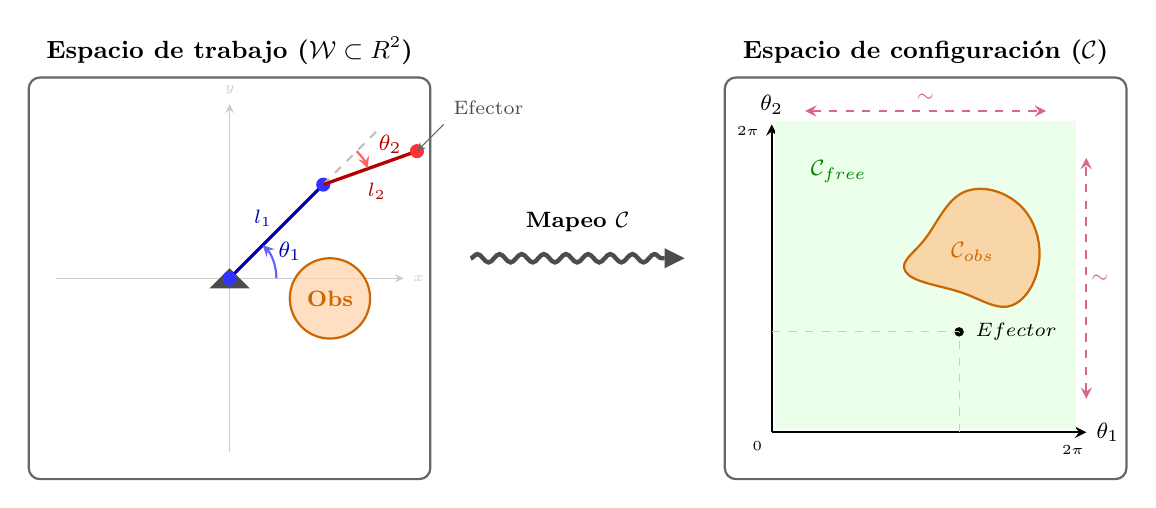
\begin{tikzpicture}[>=stealth, scale=0.85, every node/.style={font=\small}]

% =============================================
% PANEL IZQUIERDO: Espacio de Trabajo (W)
% =============================================
\begin{scope}[shift={(-5.2,0)}]
    \node[anchor=south, font=\bfseries\small] at (0, 3.05) {Espacio de trabajo ($\mathcal{W} \subset \mathbb{R}^2$)};
    \draw[rounded corners=4pt, thick, black!60] (-3.0,-3.0) rectangle (3.0,3.0);
    
    % Ejes
    \draw[->, gray!40] (-2.6,0) -- (2.6,0) node[right, font=\tiny] {$x$};
    \draw[->, gray!40] (0,-2.6) -- (0,2.6) node[above, font=\tiny] {$y$};
    
    % Base
    \fill[black!70] (-0.3,-0.15) -- (0.3,-0.15) -- (0,0.15) -- cycle;
    
    % Articulaciones (Coordenadas directas)
    \coordinate (J0) at (0,0);
    \coordinate (J1) at (1.4,1.4); % l1 a 45 grados aprox
    \coordinate (J2) at (2.8,1.9); % l2 inclinado
    
    % --- Brazo 1 ---
    \draw[very thick, blue!70!black] (J0) -- (J1);
    \fill[blue!80] (J0) circle (3pt);
    \fill[blue!80] (J1) circle (3pt);
    \node[blue!70!black, font=\scriptsize] at (0.5,0.9) {$l_1$};
    
    % Arco theta 1
    \draw[->, blue!60, thick] (0.7,0) arc (0:45:0.7);
    \node[blue!70!black, font=\footnotesize] at (0.9,0.4) {$\theta_1$};
    
    % --- Referencia Punteada (Extensión de l1) ---
    \draw[gray!50, thick, dashed] (J1) -- (2.2,2.2);
    
    % --- Brazo 2 ---
    \draw[very thick, red!70!black] (J1) -- (J2);
    \fill[red!80] (J2) circle (3pt);
    \node[red!70!black, font=\scriptsize] at (2.2,1.3) {$l_2$};
    
    % Arco theta 2 (basado en la extensión de l1)
    \draw[->, red!60, thick] (1.9,1.9) arc (45:20:0.7);
    \node[red!70!black, font=\footnotesize] at (2.4,2) {$\theta_2$};
    
    % Efector
    \draw[<-, thin, black!60] (J2) -- ++(0.4, 0.4);
    \node[font=\scriptsize, anchor=south west, black!70] at (3.2,2.3) {Efector};
    
    % Obstáculo
    \fill[orange!35, opacity=0.7] (1.5, -0.3) circle (0.6);
    \draw[orange!80!black, thick] (1.5, -0.3) circle (0.6);
    \node[font=\footnotesize\bfseries, orange!80!black] at (1.5, -0.3) {Obs};
\end{scope}

% =============================================
% FLECHA CENTRAL
% =============================================
\draw[ultra thick, black!70, decorate, decoration={snake, amplitude=1.5pt, segment length=8pt, post length=1pt}] (-1.6,0.3) -- (1.3,0.3);
\fill[black!70] (1.6, 0.3) -- (1.3, 0.45) -- (1.3, 0.15) -- cycle;
\node[anchor=south, font=\footnotesize\bfseries] at (0,0.55) {Mapeo $\mathcal{C}$};

% =============================================
% PANEL DERECHO: Espacio de Configuración (C)
% =============================================
\begin{scope}[shift={(5.2,0)}]
    \node[anchor=south, font=\bfseries\small] at (0, 3.05) {Espacio de configuración ($\mathcal{C}$)};
    \draw[rounded corners=4pt, thick, black!60] (-3.0,-3.0) rectangle (3.0,3.0);
    
    % Ejes movidos ligeramente para no chocar con el marco
    \draw[->, thick] (-2.3,-2.3) -- (2.4,-2.3) node[right, font=\footnotesize] {$\theta_1$};
    \draw[->, thick] (-2.3,-2.3) -- (-2.3,2.3) node[above, font=\footnotesize] {$\theta_2$};
    
    \node[font=\tiny, anchor=north east] at (-2.3,-2.3) {$0$};
    \node[font=\tiny, anchor=north] at (2.2,-2.35) {$2\pi$};
    \node[font=\tiny, anchor=east] at (-2.35,2.2) {$2\pi$};
    
    \fill[green!8] (-2.25,-2.25) rectangle (2.25,2.35);
    
    \fill[orange!45, opacity=0.7] 
        plot[smooth cycle, tension=0.7] 
        coordinates {(0.0,0.6) (0.6,1.3) (1.4,1.1) (1.7,0.3) (1.3,-0.4) (0.5,-0.2) (-0.3,0.1)};
    \draw[orange!80!black, thick] 
        plot[smooth cycle, tension=0.7] 
        coordinates {(0.0,0.6) (0.6,1.3) (1.4,1.1) (1.7,0.3) (1.3,-0.4) (0.5,-0.2) (-0.3,0.1)};
    
    % Etiquetas reposicionadas para visibilidad
    \node[font=\footnotesize\bfseries, orange!80!black] at (0.7,0.4) {$\mathcal{C}_{obs}$};
    \node[font=\footnotesize, green!50!black] at (-1.3,1.6) {$\mathcal{C}_{free}$};
    
    % Topología (Simetría)
    \draw[<->, dashed, purple!60, thick] (2.4,-1.8) -- (2.4,1.8);
    \node[font=\scriptsize, purple!60] at (2.6,0.0) {$\sim$};
    
    \draw[<->, dashed, purple!60, thick] (-1.8,2.5) -- (1.8,2.5);
    \node[font=\scriptsize, purple!60] at (0.0,2.7) {$\sim$};

    % --- PUNTO DE CONFIGURACIÓN ACTUAL ---
    % Elegimos una coordenada que coincida visualmente con el dibujo del brazo (ej. θ1=45°, θ2=20°)
    % En escala del C-space de -2.3 a 2.3, esto sería aprox (0.5, -0.8) 
    \fill[black] (0.5, -0.8) circle (2pt);
    \node[anchor=west, font=\scriptsize] at (0.6, -0.8) {$Efector$};
    
    % Opcional: Líneas de proyección a los ejes para mayor claridad
    \draw[gray!40, dashed, thin] (0.5, -2.3) -- (0.5, -0.8);
    \draw[gray!40, dashed, thin] (-2.3, -0.8) -- (0.5, -0.8);

\end{scope}

\end{tikzpicture}